\documentclass[10pt,a4paper]{article} 
\usepackage[utf8]{inputenc} 
\usepackage[T1]{fontenc} 
\usepackage[french]{babel} 
\usepackage{supertabular} %Nécessaire pour les longs tableaux
\usepackage[top=2.2cm, bottom=2.5cm, right=2.5cm, left=2.5cm]{geometry} %Mise en page 
\usepackage{amsmath} %Nécessaire pour les maths 
\usepackage{amssymb} %Nécessaire pour les maths 
\usepackage{stmaryrd} %Utilisation des double crochets 
%\usepackage{pifont} %Utilisation des chiffres entourés 
\usepackage{graphicx} %Introduction d images 
\usepackage{epstopdf} %Utilisation des images .eps 
\usepackage{amsthm} %Nécessaire pour créer des théorèmes 
%\usepackage{algorithmic} %Nécessaire pour écrire des algorithmes 
%\usepackage{algorithm} %Idem 
\usepackage{bbold} %Nécessaire pour pouvoir écrire des indicatrices 
\usepackage{hyperref} %Nécessaire pour écrire des liens externes 
\usepackage{array} %Nécessaire pour faire des tableaux 
\usepackage{tabularx} %Nécessaire pour faire de longs tableaux 
\usepackage{caption} %Nécesaire pour mettre des titres aux tableaux (tabular) 
\usepackage{color} %nécessaire pour écrire en couleur 
\usepackage{float} % Pour l'option [H] de \begin{figure}
\newtheorem{thm}{Théorème} 
\newtheorem{mydef}{Définition}
\newtheorem{prop}{Proposition} 
\newtheorem{lemma}{Lemme}

\newcommand{\hmm}{\textsc{HMM}}
\newcommand{\mcmc}{\textsc{MCMC}}
\newcommand{\fhmm}{\textsc{Factorial HMM}}
\newcommand{\Estep}{\textsc{E-step}}
\newcommand{\Mstep}{\textsc{M-step}}
\newcommand{\EM}{\textsc{EM}}

\title{MVA, Projet PGM : Rapport\\
  Factorial HMM}
\author{Théis \textsc{Bazin} \and Valentin \textsc{De Bortoli} \and Élie \textsc{Michel}}

\begin{document}

\maketitle

\section{Présentation du modèle}
\subsection{Comparaison avec HMM}
Le but de ce rapport est de présenter le modèle \emph{Factorial HMM}, extension du modèle \hmm, \emph{Hidden Markov Model}. Ce dernier suppose qu'une variable aléatoire cachée, dont l'évolution temporelle est régie par une chaine de Markov homogène, est à l'origine d'une observation. Le modèle que l'on se propose d'étudier ici met en parallèle $M$ chaînes de Markov homogènes et indépendantes qui sont à l'origine d'une observation. Ce modèle décrit bien à des situations d'évolution temporelle dans lesquelles plusieurs facteurs indépendants entrent en jeu. L'espace d'état de chaque variable cachée est supposé être le même et est fini de cardinal $K$. On pourrait tenter de regrouper les variables cachées en une seule variable et considérer le modèle \hmm connu. Ce modèle n'est pas satisfaisant pour deux raisons :
\begin{itemize}
\item l'espace d'état de cette unique variable cachée est alors de cardinal $K^M$, on arrive rapidement aux limites numériques des ordinateurs.
\item l'information sur l'indépendance des variables cachées est perdue.
\end{itemize}
Ces deux remarques justifient l'intérêt et la complexité de \fhmm.
\subsection{Graphe associé et inférence} 
Compte tenu de la proximité entre le modèle \fhmm et \hmm il est naturel de se poser la question de l'inférence et de la possibilité de construire un algorithme pour apprendre les paramètres du modèle. Dans ce but, on présente le graphe de \fhmm. Ce graphe permet de nouveau de mettre en évidence la complexité du nouveau modèle.
\begin{figure}[H]
\centering
\begin{minipage}{.46\linewidth}
\centering
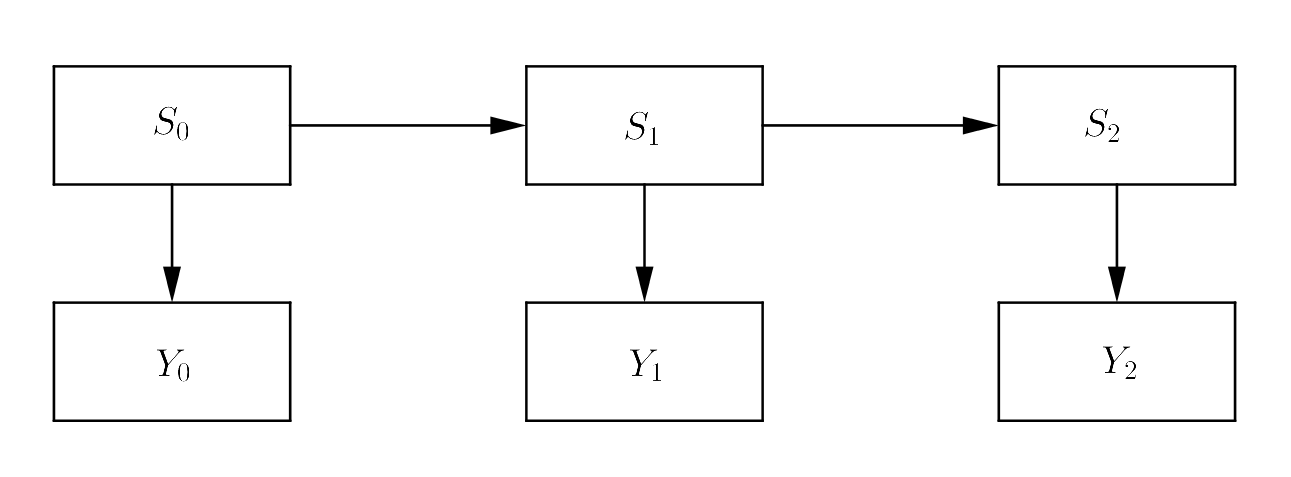
\includegraphics[scale=0.2]{graph1.png}
\caption{Modèle \hmm}
\end{minipage}
\begin{minipage}{.46\linewidth}
\centering
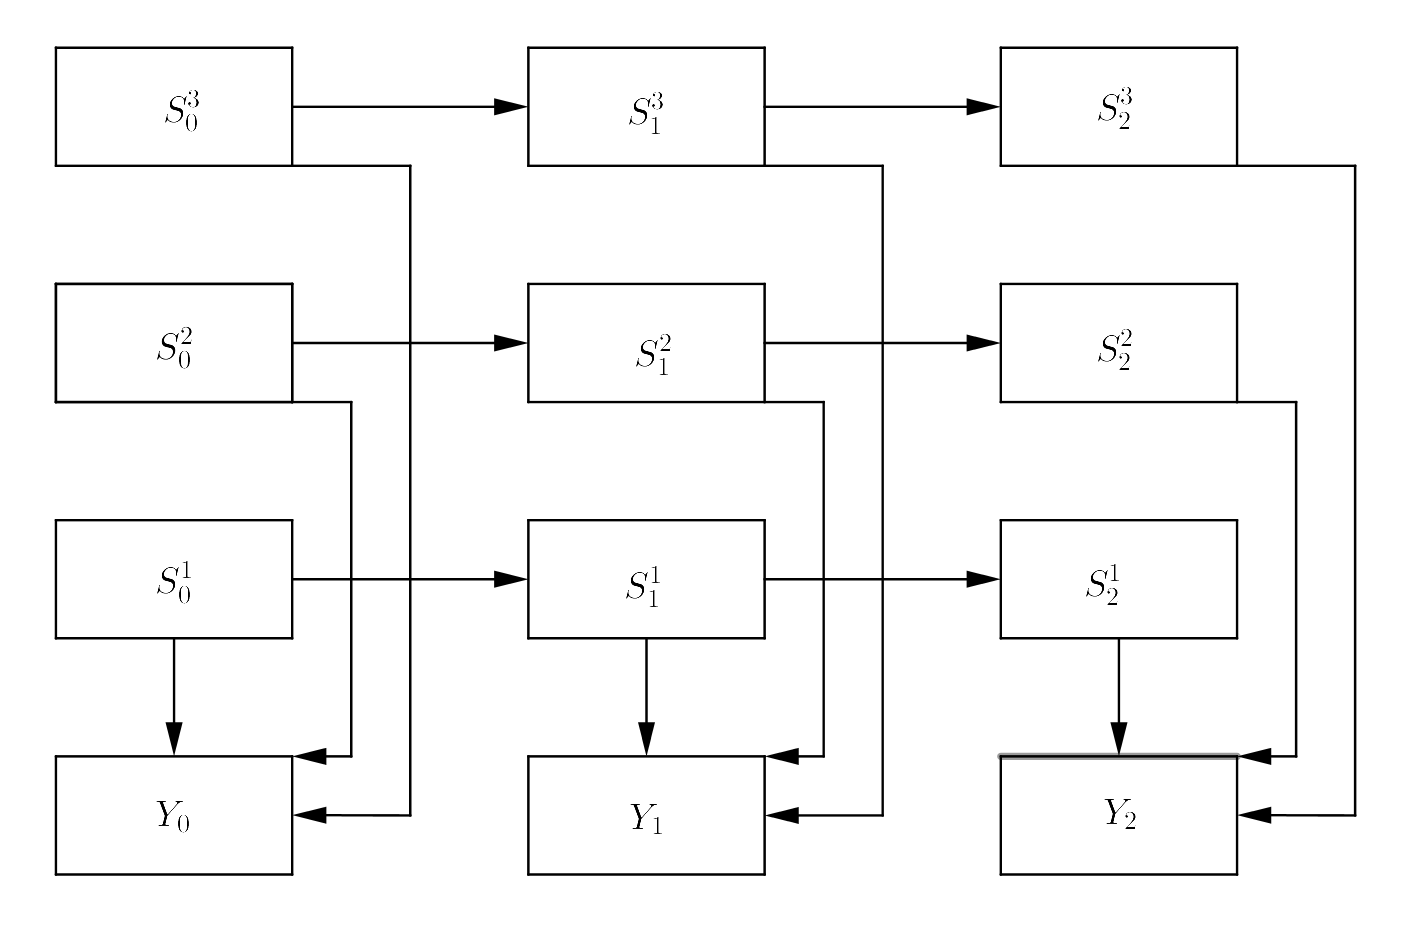
\includegraphics[scale=0.2]{graph2.png}
\caption{Modèle \fhmm}
\end{minipage}
\end{figure}
Dans le cas de \fhmm on perd la structure d'arbre. Néanmoins, on peut développer un algorithme semblable à celui développé dans \hmm qui permet de calculer exactement les marginales des probabilités se factorisant sur le graphe. Il est alors possible de résoudre exactement \Estep dans un algorithme \emph{Expectation-Maximization}, \EM. Néanmoins, cet algorithme exact n'est pas satisfaisant pour un nombre de chaînes important. On se tourne alors vers trois méthodes d'approximation :
\begin{itemize}
\item l'échantillonnage de Gibbs
\item \textit{mean-fields}
\item \textit{structured mean-fields}
\end{itemize}
Toutes ces méthodes ont été implémentées et testées sur des données génératives.
\subsection{Notations}
On fixe ici les notations qui seront utilisées dans toute la suite de notre rapport.
\newline
\begin{center}
\begin{tabular}{|c|c|} 
\hline
$T \in \mathbb{N}$ & temps de la dernière observation \\ \hline
$M \in \mathbb{N}^*$ & nombre de chaînes de Markov \\ \hline
$\Delta_K=\lbrace X \in \lbrace0,1\rbrace^K, \ \underset{k=1}{\overset{K}{\sum}}X_k=1\rbrace$ & espace d'état des variables cachées \\ \hline
$D \in \mathbb{N}^*$ & dimension des variables observées \\ \hline
$(\Pi_{k}^m)_{(m,k) \in \llbracket 1,M \rrbracket \times \llbracket 1,K \rrbracket} \in [0,1]^{MK}$ & mesures de probabilité initiales pour chaque chaîne de Markov \\ \hline
$(A_{k_1,k_2}^m)_{(m,k_1,k_2) \in \llbracket 1,M \rrbracket \times \llbracket 1,K \rrbracket^2} \in [0,1]^{MK^2}$ & matrices de transition pour chaque chaîne de Markov \\ \hline
$C \in \mathcal{S}_D^{++}(\mathbb{R})$ & matrice de covariance \\ \hline
$(W_{x,k}^m)_{(m,x,k) \in \llbracket 1,M \rrbracket \times \llbracket 1,D \rrbracket \times \llbracket 1,K \rrbracket} \in \mathbb{R}^{MDK}$ & matrices d'influence des variables cachées sur les variables observées \\ \hline
$(S_t^m)_{(m,t) \in \llbracket 1,M \rrbracket \times \llbracket 0,T \rrbracket } \in \Delta_K^{(T+1)\times M}$ & variables cachées \\ \hline
$(Y_t)_{t \in \llbracket 0,T \rrbracket} \in \mathbb{R}^D$ & variables observées \\ \hline
\end{tabular}
\end{center}

Les différentes contraintes (sommation à 1) sur les mesures de probabilité n'ont pas été rappelées ici. Pour plus de simplicité on notera $Y_{(t)}$ le vecteur $(Y_t)_{t \in \llbracket 0,T \rrbracket}$, $Y_{(-t)}$ le vecteur $(Y_{t})_{t \in \llbracket 0,T \rrbracket\backslash \lbrace t \rbrace}$, $Y_{(t_1,t_2)}$ le vecteur $(Y_t)_{t \in \llbracket t_1,t_2 \rrbracket}$. Ces notations s'étendent aux variables cachées. Enfin on notera $\theta=(\Pi, A,C,W)$ le vecteur de paramètres.
\section{Le problème d'inférence et l'algorithme EM}
\subsection{Algorithme EM}
Soit $p$ une mesure de probabilité qui se factorise selon \fhmm. On a alors :
\begin{multline}
p(S_{(t)}^{(m)},Y_{(t)} \vert \theta)=\underset{m=1}{\overset{M}{\prod}}\underset{k=1}{\overset{K}{\prod}}(\Pi_k^m)^{(S_0^m)_k}\underset{t=1}{\overset{T}{\prod}}\underset{m=1}{\overset{M}{\prod}}\underset{k_1=1}{\overset{K}{\prod}}\underset{k_2=1}{\overset{K}{\prod}}(A_{k_1,k_2}^m)^{(S_t^m)_{k_2}(S_{t-1}^m)_{k_1}}\\ \underset{t=0}{\overset{T}{\prod}}\frac{1}{(2\pi)^{D/2}}\frac{1}{\vert C  \vert^{1/2}}\exp\left(-1/2 {}^t\left(Y_t- \underset{m=1}{\overset{M}{\sum}}W^m S_t^m \right)C^{-1} \left(Y_t- \underset{m=1}{\overset{M}{\sum}}W^m S_t^m \right)\right) \label{jointprob}
\end{multline}
De manière analogue au cas \hmm ou \textsc{Gaussian mixture} il n'est pas facile de calculer $p(Y_{(t)})$. L'algorithme \EM est une méthode itérative qui permet de considérer seulement la probabilité jointe \ref{jointprob} dont la forme est facile à manipuler. L'idée est la suivante :
\begin{equation}
\begin{aligned}
p(Y_{(t)})&=\int_{S_{(t)}^{(m)}}p(S_{(t)}^{(m)},Y_{(t)}) \\
&=\int_{S_{(t)}^{(m)}}\frac{p(S_{(t)}^{(m)},Y_{(t)})}{q(S_{(t)}^{(m)})}q(S_{(t)}^{(m)}) \\
&=\mathbb{E}_q\left(p(S_{(t)}^{(m)},Y_{(t)}) \right)
\end{aligned}
\end{equation}
Si on considère la log-vraisemblance on peut utiliser l'inégalité de Jensen et on obtient :
\begin{equation}
\begin{aligned}
l(Y_{(t)},\theta)&=\log(p(Y_{(t)}) \\
&=\log\left( \mathbb{E}_q\left(p(S_{(t)}^{(m)},Y_{(t)}) \right) \right)
&\ge \mathcal{L}(Y_{(t)},\theta,q)
\end{aligned}
\end{equation}
Avec $\mathcal{L}(Y_{(t)},\theta,q)=\mathbb{E}_q \log \left( p(S_{(t)}^{(m)}, Y_{(t)})\right)+H(q)$ où $H(q)$ est l'entropie de $q$. Il s'agit alors de maximiser cette log-vraisemblance approchée en $q$ et en $\theta$. La maximisation à $\theta$ fixé implique 
\begin{equation}
\hat{q}=p(S_{(t)}^{(m)} \vert \theta,Y_{(t)}^{(m)})
\end{equation} 
Une autre conséquence est l'égalité suivante :
\begin{equation}
\mathcal{L}(Y_{(t)},\theta,\hat{q})=l(Y_{(t)},\theta) \label{increase}
\end{equation}
L'algorithme consiste à appliquer un algorithme de Gauss-Seidel avec contraintes sur la log-vraisemblance approchée, les deux variables considérées étant $q$ \footnote{$q$ peut être vue comme une mesure de probabilité mais d'un point de vue optimisation on considère $q$ comme une variable de $[0,1]^{K^M}$} et $\theta$. On distingue ainsi deux étapes :
\begin{itemize}
\item \Estep : $q_{n+1}=p(S_{(t)}^{(m)} \vert \theta_n,Y_{(t)}^{(m)})$
\item \Mstep : maximisation de $\mathbb{E}_{q_n} \left( \log \left( p(S_{(t)}^{(m)}, Y_{(t)}  \vert  \theta )\right) \right)$
\end{itemize}
Les conditions initiales n'ont pas été discutées ici. Néanmoins elles jouent un rôle crucial dans cet algorithme au comportement très local. En effet, très peu de résultats assurent la convergence théorique de cet algorithme vers un maximum local. Dans \cite{wu1983convergence}, les auteurs montrent que sous certaines conditions on a l'assurance de la convergence vers un point stationnaire. Les conditions de maximalité sont plus dures à obtenir. Il est cependant important de remarquer que \ref{increase} assure une croissance de la log-vraisemblance à chaque étape de l'algorithme.
\subsection{M step}
On détaille désormais l'étape \Mstep de notre algorithme. On rappelle qu'il s'agit de maximiser $\mathcal{L}_{approx}(\theta)=\mathbb{E}_{q_n}\left( \log \left( p(S_{(t)}^{(m)},Y_{(t)}\vert \theta)\right)\right)$. La maximisation selon $(\Pi_{k}^m)_{(m,k) \in \llbracket 1,M \rrbracket \times \llbracket 1,K \rrbracket}$ (respectivement selon $(A_{k_1,k_2}^m)_{(m,k_1,k_2) \in \llbracket 1,M \rrbracket \times \llbracket 1,K \rrbracket^2}$) pouvant se faire indépendamment des autres variables, on obtient après utilisation des multiplicateurs de Lagrange\footnote{Le fait que l'on travaille sur des ouverts, i.e $\Pi_{k}^m$ et $A_{k_1,k_2}^m$ ne s'annulent jamais, n'est pas détaillé ici. Cette propriété est issue de la divergence du logarithme en $0$}.
\begin{equation}
\widehat{\Pi_k^m}=q_{n}((S_0^m)_k=1)
\end{equation}
De même on obtient.
\begin{equation}
\widehat{A_{k_1,k_2}^m}=\frac{\underset{t=1}{\overset{T}{\sum}}q_n((S_{t-1}^m)_{k_1}=1,(S_t^m)_{k_2}=1)}{\underset{t=1}{\overset{T}{\sum}}q_n((S_{t-1}^m)_{k_1}=1)}
\end{equation}
Pour la suite, on note $W \in \mathcal{M}_{DM,K}(\mathbb{R})$ la matrice obtenue en concaténant les matrices $(W_m)_{m \in \llbracket 1,M \rrbracket}$. De la même manière on note $S_t$ le vecteur obtenu en concaténant tous les vecteurs $(S_t^m)_{m \in \llbracket 1,M \rrbracket}$. Il s'agit alors de maximiser en $(W,C)$ la fonction suivante $\mathcal{L}'(W,C)=\mathbb{E}_{q_n}\left(-\frac{T+1}{2} \log(\vert C \vert) -\frac{1}{2} {}^t\left(Y_t-WS_t \right)C^{-1} \left( Y_t-WS_t\right)\right)$. Cette étude est classique (maximisation des paramètres pour la log-vraisemblance d'une gaussienne) et les calculs ont déjà été effectués à plusieurs reprises. On rappelle simplement que la maximisation se fait d'abord sur $W$, l'argument maximum ne dépendant pas de $C$ on peut facilement réinjecter dans $\widehat{W}$ dans $\mathcal{L}'(\widehat{W},C)$ et optimiser selon $C$\footnote{En réalité on optimise selon $C^{-1}$ qui donne une expression plus facile à manipuler}. On obtient les expressions suivantes :
\begin{equation}
\widehat{W}=\left( \underset{t=0}{\overset{T}{\sum}} Y_t \times \mathbb{E}_{q_n}({}^tS_t) \right) \left( \underset{t=0}{\overset{T}{\sum}} \mathbb{E}_{q_n}\left( S_t {}^t S_t\right)\right)^+
\end{equation}
Où $M^+$ est la pseudo-inverse de Moore-Penrose. On a ici utilisé le fait que la pseudo-inverse de Moore-Penrose donne une solution au problème des moindres carrés CITER. La maximisation selon $C^{-1}$ donne :
\begin{equation}
\widehat{C}=\frac{1}{T+1}\underset{t=0}{\overset{T}{\sum}}Y_t {}^tY_t-\frac{1}{T+1}\underset{t=0}{\overset{T}{\sum}}\underset{m=1}{\overset{M}{\sum}}W^m\mathbb{E}_{q_n}(S_t^m){}^t Y_t
\end{equation}
On remarque que les mises à jour données par \Mstep dépendent de \Estep uniquement pour le calcul de trois quantités :
\begin{itemize}
\item $\forall (t,m) \in \llbracket 0, T\rrbracket \times \llbracket 1,M \rrbracket, \ \mathbb{E}_{q_n}(S_t^m) $
\item $\forall (t,m_1,m_2) \in \llbracket 0, T\rrbracket \times \llbracket 1,M\rrbracket^2, \ \mathbb{E}_{q_n}(S_t^{m_1}S_t^{m_2}) $
\item $\forall t \in \llbracket 1,T \rrbracket \times \llbracket 1,M \rrbracket, \ \mathbb{E}_{q_n}(S_{t-1}^mS_t^{m})$
\end{itemize}
On rappelle que les multiplications considérées ici le sont élément par élément. Il s'agit donc de calculer ces trois quantités afin de pouvoir les réinjecter dans \Mstep. Pour cela, on considère une méthode d'inférence exacte deux méthodes d'inférences variationnelles et une méthode d'échantillonnage.
\section{E step}
\subsection{Inférence exacte}
Pour présenter cet algorithme il est bon d'avoir à l'esprit les calculs effectués lors de la récurrence alpha-beta de \hmm. Les calculs sont très semblables.
Le problème est ici plus complexe puisque l'on n'a plus une chaîne de Markov mais $M$. On pose :
\begin{equation}
\left\lbrace
\begin{aligned}
&\alpha_t=p(S_t^{1},\dots,S_t^{M},Y_{(1,t)}\vert \theta) \\
&\forall m \in \llbracket 1,M \rrbracket, \ \alpha_t^m=p(S_{t-1}^1, \dots, S_{t-1}^m,S_{t}^{m+1}, \dots, S_{t}^M, Y_{(1,t-1)} \vert \theta) \\
&\beta_t=p(Y_{(t+1,T)} \vert S_t^1, \dots,S_t^M, \theta) \\
&\forall m \in \llbracket 1,M \rrbracket, \ \beta_t^m=p(Y_{(t,T)} \vert S_t^1, \dots, S_t^m,S_{t-1}^{m+1}, \dots, S_{t-1}^M, \theta)
\end{aligned}
\right.
\end{equation}
On remarque que :
\begin{equation}
\left\lbrace 
\begin{aligned}
&\forall t \in \llbracket 1,T \rrbracket, \ \alpha_{t-1}=\alpha_{t}^M  \\
&\forall t \in \llbracket 0,T \rrbracket, \ \beta_{t}=\beta_{t}^0
\end{aligned}
\right.
\end{equation}
Quatre autres équations permettent de compléter la récurrence :
\begin{equation}
\left\lbrace
\begin{aligned}
&\alpha_t=p(Y_t \vert S_t^{(m)}, \theta)\alpha_t^0 \\
&\forall m \in \llbracket 0,M-1 \rrbracket, \ \alpha_t^m=\underset{S_{t-1}^{m+1}}{\sum}p(S_t^{m+1} \vert S_{t-1}^{m+1}, \theta) \alpha_t^{m+1} \\
&\beta_{t-1}^M=P( Y_t \ \vert S_t^{(m)},\theta) \beta_t \\
&\forall m \in \llbracket 0, M-1 \rrbracket, \ \beta_t^{m}=\underset{S_{t+1}^{m+1}}{\sum}p(S_{t+1}^{m+1} \vert S_{t}^{(m+1)}, \theta) \beta_{t}^{m+1}
\end{aligned}
\right.
\end{equation}
On obtient le schéma suivant :
\begin{figure}[H]
\centering
\begin{minipage}{.46\linewidth}
\centering
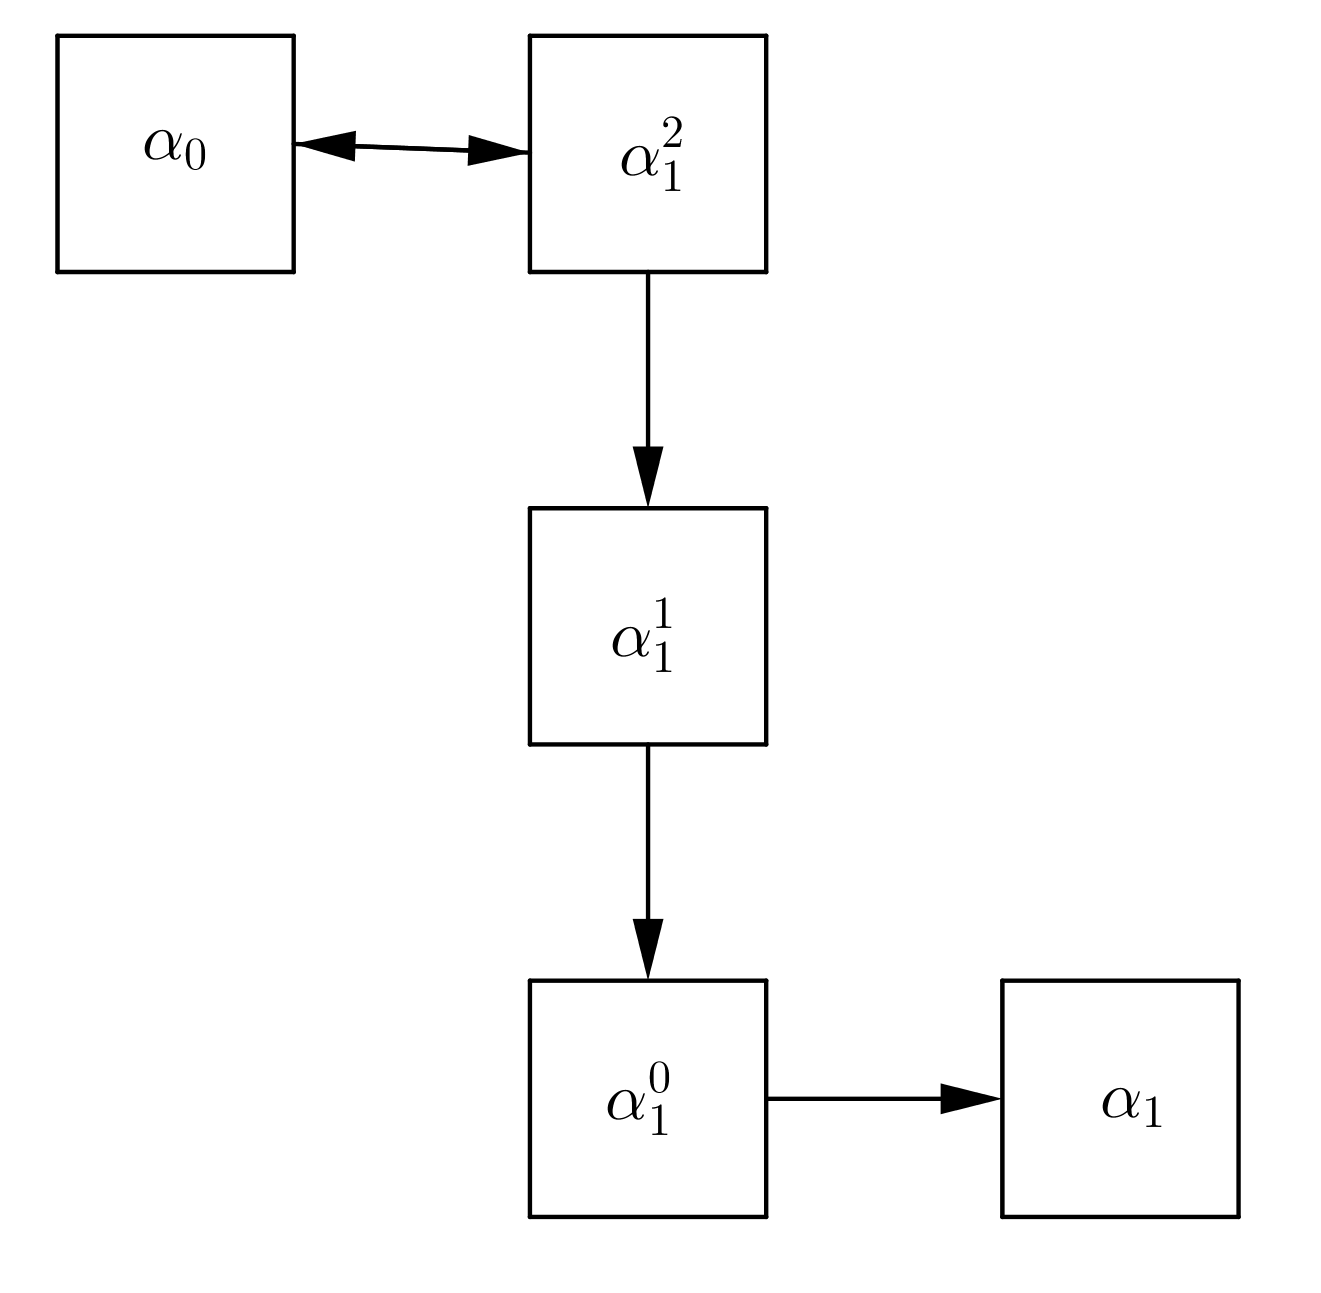
\includegraphics[scale=0.2]{graph3.png}
\caption{Récurrence sur $\alpha$}
\end{minipage}
\begin{minipage}{.46\linewidth}
\centering
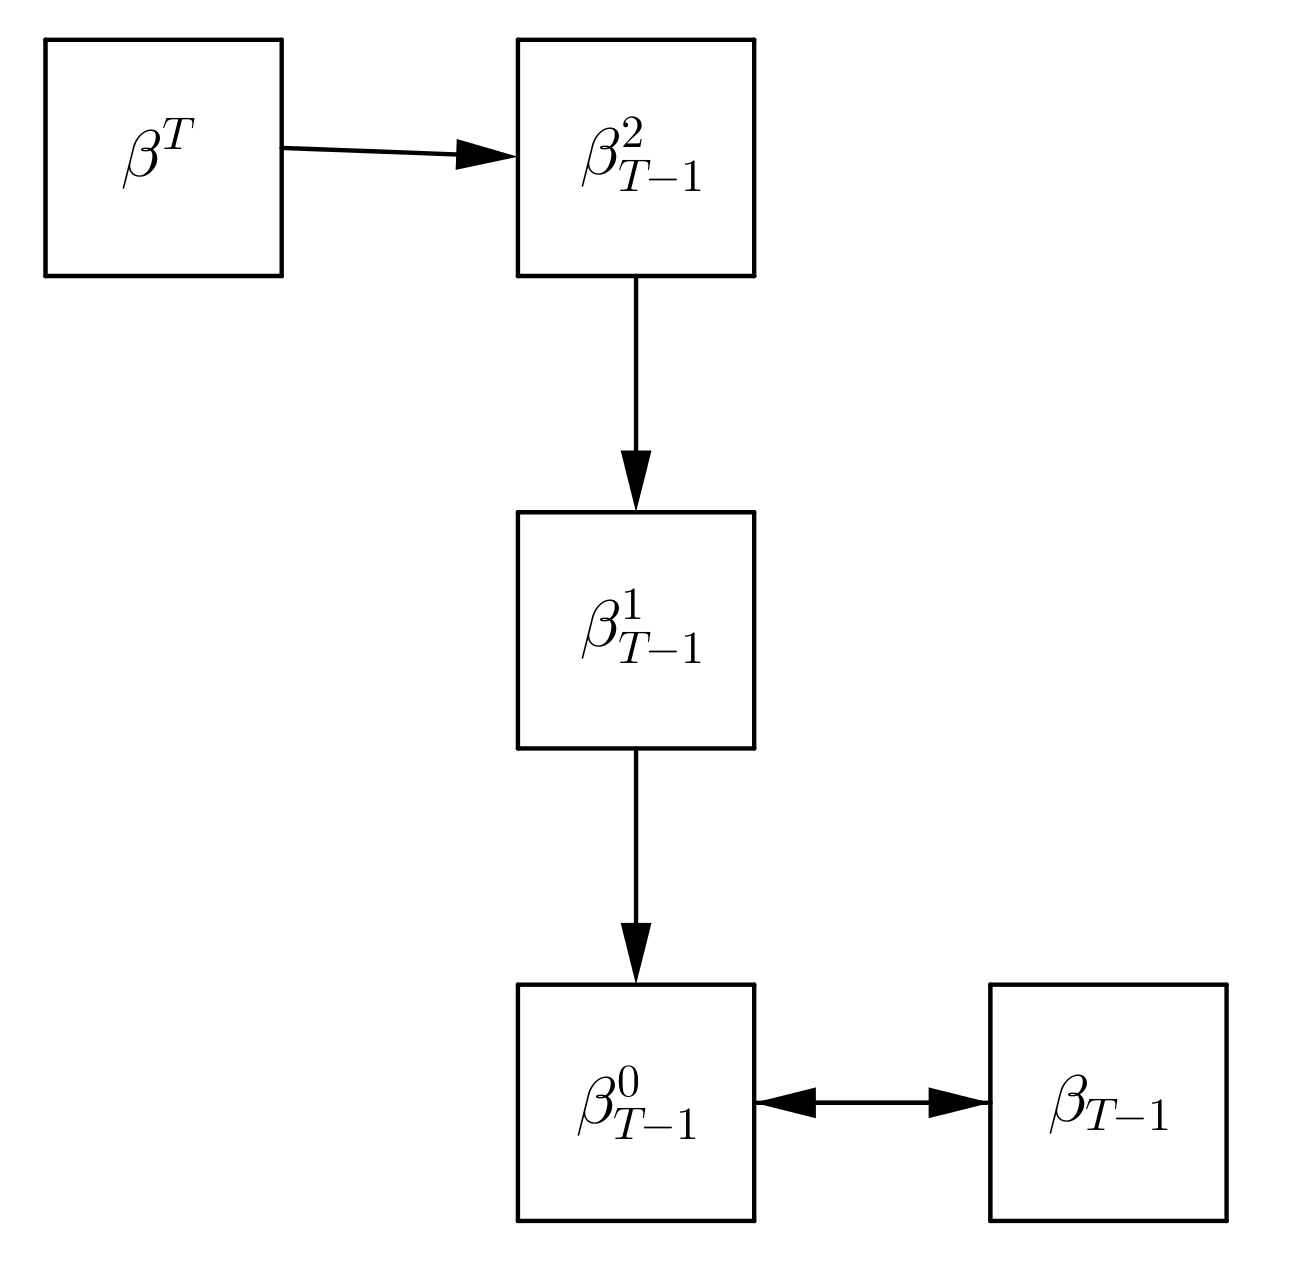
\includegraphics[scale=0.2]{graph4.png}
\caption{Récurrence sur $\beta$}
\end{minipage}
\end{figure}
On peut alors calculer $\gamma_t$ de la manière suivante :
\begin{equation}
\gamma_t=p(S_t \vert Y_{(t)}, \theta)= \frac{\alpha_t \beta_t}{\underset{S_t}{\sum} \alpha_t \beta_t}
\end{equation}
Il convient alors de calculer les trois quantités issues de \Mstep :
\begin{itemize}
\item $\mathbb{E}_{q_n}(S_t^m)= \underset{S_t^n, \ n \neq m}{\sum} \gamma_t$
\item $\mathbb{E}_{q_n}(S_t^{m_1}S_t^{m_2})= \underset{S_t^n, \ n \neq m_1, \ n \neq m_2}{\sum} \gamma_t$
\item $\mathbb{E}_{q_n}(S_{t-1}^mS_t^m)= \frac{\underset{S_{t-1}^n,S_t^r, \ n \neq m, \ r \neq m}{\sum}\alpha_{t-1} p(S_t \vert S_{t-1}) p(Y_t \vert S_t) \beta_t}{\underset{S_{t-1}, S_t}{\sum}\alpha_{t-1}p(S_t \vert S_{t-1})p(Y_t \vert S_t) \beta_t} $
\end{itemize}
Il est important de préciser que les formules données sont exactes seulement lorsqu'elles sont appliquées en un point. En effet, $\alpha_t, \beta_t, \gamma_t$ sont des éléments de $\mathbb{R}^{\llbracket 1,K \rrbracket^M}$. Pour plus de détails sur le sens de ces formules on renvoie à l'implémentation en Python de cet algorithme \href{url}{https://github.com/eliemichel/fHMM}.
\subsection{Échantillonnage de Gibbs}
L'inférence exacte peut être très assez couteuse en terme d'opérations ($\mathcal{O}(TMK^{M+1})$). L'algorithme d'échantillonnage de Gibbs fournit lui un moyen d'échantillonner approximativement selon $p(S_{(t)}^{(m)} \vert Y_{(t)}, \theta)$ mais de manière rapide. En effet, l'échantillonnage de Gibbs peut être vu comme un cas particulier de \emph{Monte Carlo Markov Chain}, pour laquelle la convergence en probabilité est assurée. Néanmoins, on ne possède pas d'information sur la vitesse de convergence de ces algorithmes vers la probabilité voulue. Le choix des auteurs de \cite{ghahramani1997factorial} a été de ne pas prendre en compte le temps de mise en route de l'échantillonneur de Gibbs et de directement sélectionner les premiers échantillons produits par l'algorithme. Ce choix sera discuté par la suite. On précise le déroulement de l'échantillonnage :
\begin{itemize}
\item les différents états $S_{(t)}^{(m)}$ sont initialisés selon une loi uniforme sur $\llbracket 1,K \rrbracket$.
\item les états $S_0^{(m)}$ sont mis à jour de manière successive (d'abord $S_0^1$ tiré selon $p(S_0^1 \vert Y_{0}, S_1^1, S_0^{(-1)}$, puis $S_0^2$ tiré selon $p(S_0^2 \vert Y_{0}, S_1^2, S_0^{(-2)}$).
\item les états $S_t^{(m)}$ sont mis à jour de manière successive pour $t \in \llbracket 1,T$
\item on extrait l'échantillon. Les opérations sont répétées $N_s$ fois à partir de la seconde étape pour obtenir autant d'échantillons de Gibbs.
\end{itemize}
On détaille simplement le calcul de la probabilité pour $t \in \llbracket 1,T-1 \rrbracket$ (les autres calculs sont similaires).
\begin{equation}
\begin{aligned}
p(S_t^m \vert Y_t, S_{(t)}^{(m)} \backslash S_t^m)&=\frac{1}{Z_1}p(S_t^{m}, S_{(-t)}^{m}, S_{t}^{(-m)},Y_t) \\
&=\frac{1}{Z_2}p(Y_t \vert S_t^{m},S_t^{(-m)}) p(S_t^m \vert S_{t-1}^m) p(S_{t+1}^m \vert S_t^m)
\end{aligned}
\end{equation}
La constante $Z_2$ est facilement calculable en sommant en notant que $\underset{S_t^m}{\sum}p(S_t^m \vert Y_t, S_{(t)}^{(m)} \backslash S_t^m)=1$.
\bibliographystyle{plain}
\bibliography{reportbib}
\end{document}